%%%%%%%%%%%%%%%%%%%%%% IMPORTANT INFO %%%%%%%%%%%%%%%%%%%%%%%%%%%%%%
% SRAM read/write latency is in the order of 8ns 		 [ Intermittent computation without hardware support of programmer intervention]
% FRAM read/write latency is in the orfer of 60ns/100ns  [Texas Instrument MSP430FR573x DataSheet]
%%%%%%%%%%%%%%%%%%%%%%%%%%%%%


Advances in processor efficiency along with the development of
energy-harvesting systems has created a new category of devices that require
neither a battery nor a tethered power
supply~\citep{prasad_comst_2014,lucia_snapl_2017,soyata_csm_2016}. These
devices operate using ambient energy, such as radio frequency
transmissions~\citep{rf_powered_computing_gollakota_2014},
light~\citep{margolies_infocom_2016,margolies_tosn_2016}, and
vibration~\citep{gorlatova_sigmetrics_2014}. Incorporating compute, storage,
sensing, and communication hardware~\citep{wisp5,moo,capybara}, such devices are a
promising technology for use in the Internet of Things~\citep{ku_cst_2016},
in-body~\citep{nadeau_naturebio_2017} and
on-body~\citep{bandodkar_electroanalysis_2015} medical systems, and
energy-harvesting nano-satellites~\citep{kicksat,capybara}.

Energy-harvesting devices create unique challenges because they operate {\em
intermittently} when energy is
available~\citep{hicks_isca_2017,lucia_snapl_2017}. An energy-harvesting device
buffers energy in a small storage capacitor~\citep{gorlatova_tmc_2013,gunduz_commag_2014} and operates when a
threshold amount of energy has accumulated. Harvestable energy sources are low-power (e.g., nW to $\mu$W) compared to a platform's operating
power level (hundreds of $\mu$W to mW). A device operates briefly until it depletes its buffered energy, after which, the device shuts
down and recharges to operate again later. As an example, recharge times may be
tens of seconds in radio frequency powered medical device~\cite[Fig.
3c]{nadeau_naturebio_2017}.  The recharge and discharge time---which corresponds to the device's inactive and active time---varies with the energy buffering capacitor's~\cite{capybara} and some devices fail and restart operating $\approx$10 to
$\approx$100 times per second~\citep{tan_infocom_2016,mementos,nvp}.

\begin{wrapfigure}{t!}{0.5\textwidth}
    \centering
    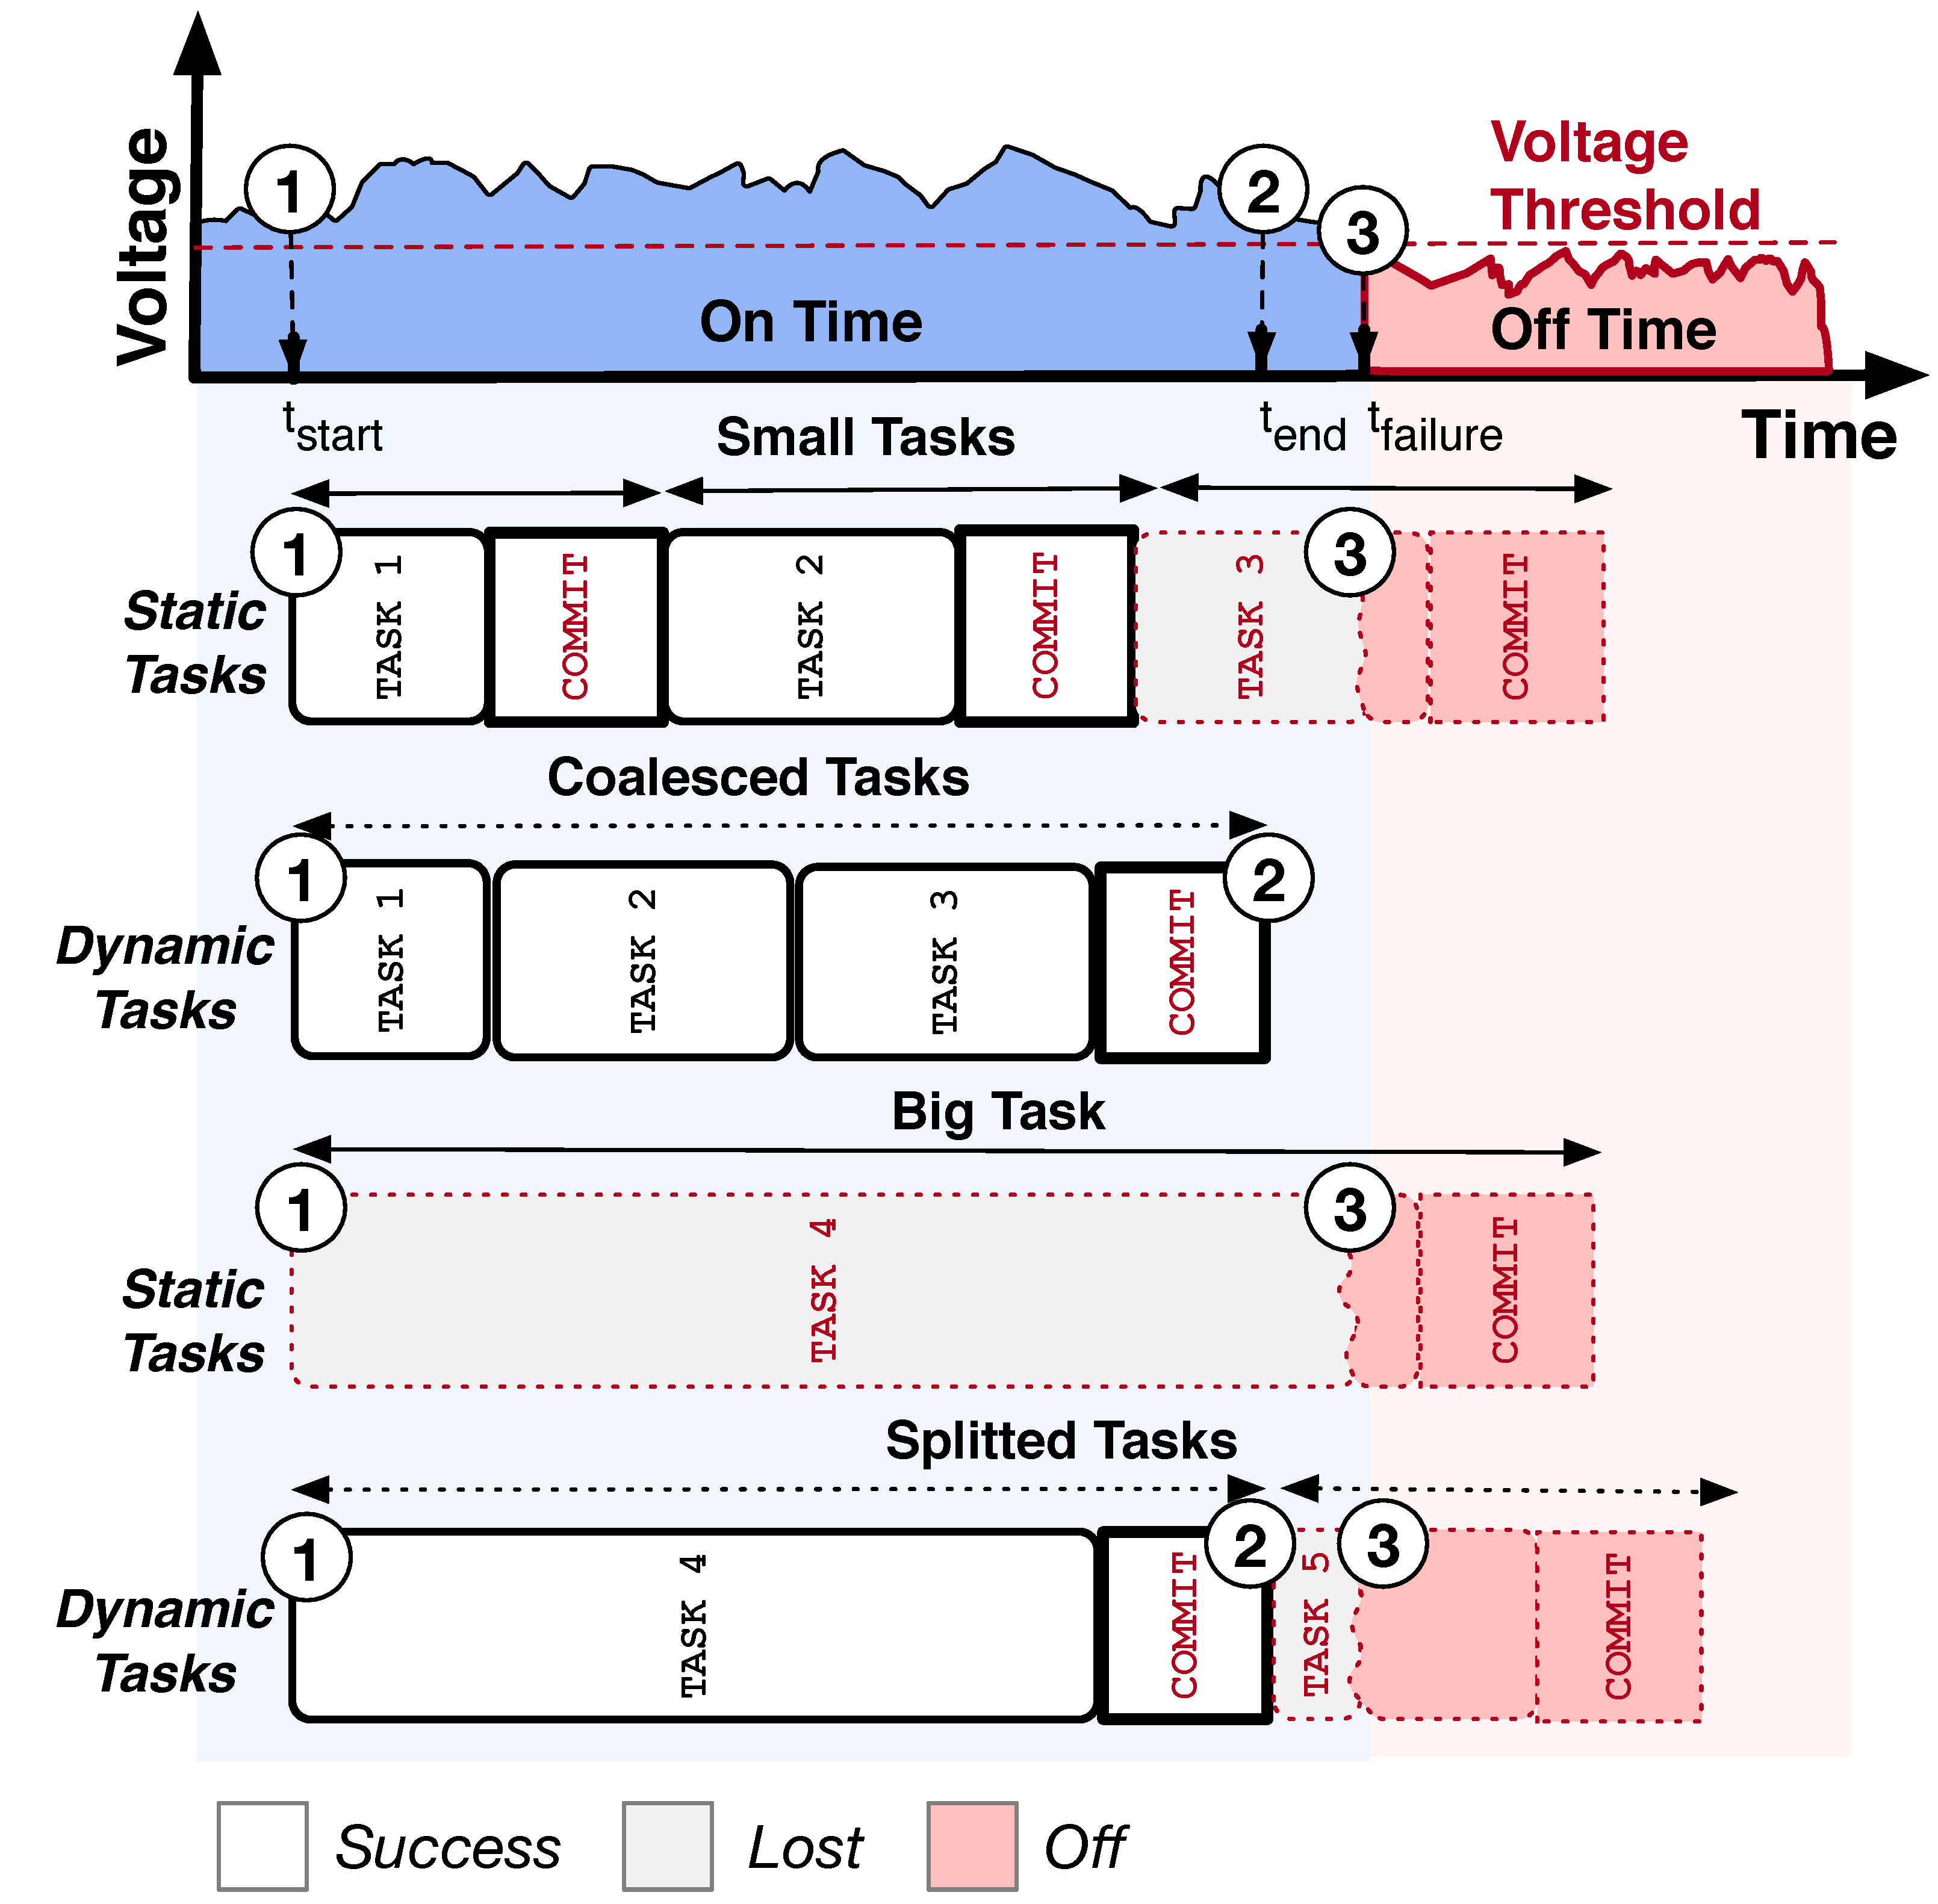
\includegraphics[width=0.5\textwidth]{figures/graffle/intro-figure.pdf}
    \caption{Task coalescing at runtime reduces time and energy overhead in task-based intermittent programming models by performing fewer commits and buffering updates to non-volatile (NV) variables in volatile (V) memory.}
    \label{fig:coalesce}
\end{wrapfigure}

\textbf{Data Consistency in Intermittent Computing.}  Software in an
energy-harvesting system operates according to the {\em intermittent execution
model}~\citep{dino,lucia_snapl_2017}, which corresponds to the
operation-failure-restart cycles of an energy-harvesting device. In an
intermittent software execution, an {\em operating period} proceeds for an
arbitrary duration (dictated by energy availability) before being interrupted
by a {\em failure period}. In a failure period, a device loses the volatile
state in its registers, stack, SRAM, and retains the state of any non-volatile
memory, such as FRAM or Flash. While capturing periodic
checkpoints~\citep{mementos,quickrecall} and sleep
scheduling~\citep{dewdrop,hibernus,hibernusplusplus} help preserve execution
progress, failures can leave non-volatile state incorrectly, partially updated,
and may leave checkpointed volatile state inconsistent with non-volatile state.
These inconsistencies cause intermittent execution to deviate from
continuously-powered behavior, often leading to an unrecoverable
application failure~\citep{dino,edb}. 

Prior work developed two main approaches to dealing with data inconsistency for
intermittently-powered devices: (i) \emph{software-based programming and
execution models}~\citep{dino,ratchet,chain,alpaca} and (ii)
\emph{hardware-based computer architecture
support}~\citep{hicks_isca_2017,idetic,nvp}.  Complex architectural changes are
expensive to design, verify, and manufacture.  New architectures are also
inapplicable to existing systems~\citep{hicks_isca_2017,nvp}. Software
approaches are simpler and applicable to existing devices today, but prior
software approaches have a number of limitations that are the focus of the work
in this paper.  A key limitation of prior software approaches that we address in this paper is the {\em inflexibility} of a program statically decomposed into tasks. 

\textbf{Task Decomposition of Intermittent Programs.} {\em
Task-based} programming and execution models require a
programmer~\citep{alpaca,chain} or a compiler~\cite{baghsorkhi_cgo_2018} to
statically decompose a program into a collection of {\em tasks}.  A task can
include arbitrary computation and these existing systems guarantee that each
tasks executes {\em atomically}, despite arbitrarily-timed power failures.  
%
The programmer explicitly expresses task-to-task control flow, or the compiler
converts existing program control-flow into task-to-task control flow to sequence 
the tasks that it defines.
%
Figure~\ref{fig:coalesce} (top) illustrates how a program's tasks execute and
shows how tasks can impose a run-time overhead. 
%
At each task transition, the system incurs an overhead to track and atomically
commit modifications to the non-volatile memory, to maintain consistency of
program state~\citep{chain,alpaca}.  
%
The more task transitions a program executes at run time, the more overhead.

A savvy programmer may thus create very large tasks in an attempt to minimize
overhead by minimizing the number of task transitions.  However, a very large
task may require more energy to complete than a device's fixed hardware energy
buffer can hold.  Such a large task fails to completely execute assuming only
buffered energy is available (i.e., assuming the worst case).  While some
environments may have sufficient harvestable energy to replenish a device's
capacitor during operation, prolonging the execution period and enabling the
task to complete, assuming cooperation from the physical environment to avoid
non-termination is a risky programming proposition.  To eliminate this risk,
existing systems require the programmer or compiler to decompose a  program
into small tasks, all of which complete using only buffered energy.  These
constraints on task sizing leave an unsatisfying dilemma: large, efficient
tasks that risk non-termination, or small tasks that are guaranteed to
complete, but incur a high task transition and commit overhead.  In this work,
we propose a third way, using a novel technique called {\em dynamic task
coalescing} that efficiently executes small tasks, avoiding unnecessary
overheads while avoiding the risk of non-termination.

%A key challenge is that the length of a software
%task's execution is \emph{limited by the fixed total amount of energy} that a
%device can buffer in hardware. A task's code is static, but the duration of its
%execution may be input-dependent and is difficult to predict. To illustrate
%this, we refer to Figure~\ref{fig:1} showing the execution time of two
%applications (the same application X, but divided into X and Y tasks as
%in~\citep{chain}) running on RFID antenna-powered Computational
%RFID~\citep{wisp,rf_powered_computing_gollakota_2014} at two device-to-antenna
%distances (near---stable energy supply/far---high energy intermittency). At
%short distance: execution will takes too long caused by runtime cost of
%marshalling excessively small tasks. At far distance: program \emph{might never
%execute} if task execution consumes more energy than the system can buffer.
%This calls for at-runtime adaptive task division of any transiently-powered
%application---namely \emph{task virtualization}.

In this work, we introduce a new system called \sys, which executes a task-based
intermittent program by dynamically coalescing its tasks.
\sys accepts any static decomposition (i.e., from the programmer or from a compiler) 
and coalesces its tasks at runtime. Two consecutive, coalesced tasks execute  
with no commit or task transition overhead between them, instead performing
task-end commit actions at the end second task only.
%
When there is sufficient energy to execute both tasks, two distinct, small
tasks are effectively executed as a single large task, preserving the atomicity
of both.  If power fails during a coalesced task, execution restarts from the
{\em first} of the coalesced tasks.  Figure~\ref{fig:coalesce} (bottom)
illustrates how dynamic coalescing changes the earlier execution and highlights
the change in memory model necessary to not break atomicity.

%Brandon: This is too detailed for the intro:
%Unfortunately, naively merging two atomic tasks might produce a non-atomic
%task, that may leave non-volatile memory inconsistent after a partial
%execution. A merge breaks atomicity when atomic merged tasks form a
%\emph{write-after-read (WAR)} dependency---for instance if two tasks
%\texttt{\{x=y+1\}; \{y=x;\}} are merged and if the power failure occurs after
%\texttt{x=y}, the value \texttt{x} will be increased twice when the merged task
%is restarted, that leads to an inconsistency.

%variables in non-volatile memory at \emph{run-time} that can
%break the atomicity of the \emph{virtual task}. Consider the
%example depicted in Fig.~\ref{fig:virtualization}: Tasks 1,
%2 and 3 being executed consecutively. All tasks in this
%example are atomic since they do not have WAR dependency on
%the persistent variables they are accessing, e.g. \emph{x}
%is only read and \emph{y} is only written within Task 1.
%Now, suppose three tasks have been virtualized into a single
%one at run-time, namely Task 4: since \emph{x} is now first
%\emph{read} and then \emph{written}, a WAR dependency on
%\emph{x} is introduced dynamically at
%run-time---unfortunately Task 4 is \emph{no more atomic}
%since its re-execution will not always produce the same
%results.

While a compiler can use static data privatization and commit instrumentation
(i.e., redo-logging) to eliminate statically identifiable, inter-task data
dependences~\citep{alpaca}, a \emph{dynamic} dependence between two coalesced
tasks requires dynamic privatization and commit actions. 
%
To ensure consistency and respect inter-task dependences, \sys uses a novel
approach to \emph{memory virtualization} that buffers non-volatile variable
updates in volatile memory during coalesced task execution, before committing
them to non-volatile memory at the dynamic task boundary.
%
%Therefore, we require a \emph{new execution
%model} that keeps each virtual task atomic by committing the
%modified persistent variables at the boundary defined
%dynamically at run-time---keeping the non-volatile memory
%unmodified upon a power-interrupt and preserving its
%consistency.

A static task decomposition model assumes that each
single task can execute to completion.  If the hardware energy buffer provides
inadequate energy to execute each single task to completion, a program will not
terminate~\cite{cleancut_2018}. To avoid non-termination under adversarial 
energy conditions, \sys uses a timer-based {\em partial task commit} mechanism.
Partial commit avoids non-termination by committing the intermediate state of a long-running
task that has repeatedly failed and restarted.  Partial commit violates
task atomicity, but preserves forward progress; if a programmer knows that
task atomicity is crucial to correctness, they can disable partial commit
instead risking non-termination.

%Task coalescing removes the burden from the programmer, because it accepts any
%task decomposition and improves it dynamically. To further reduce the
%programmer effort, we propose a compiler pass for \emph{automatic
%decomposition} of programs into (small) \emph{atomic} tasks. The compiler
%identifies non-volatile variables shared across tasks as tasks are created, and
%instruments reads and writes of those variables, using memory virtualization,
%to keep the data consistent in the presence of power loss.
%
%\textcolor{red}{Despite being limited to a subset of the C language, the
%automatic task decomposition allowed us to port several	applications to an
%intermittent platform with a moderate effort.}

\textbf{Contributions.} To summarize, \sys's main contributions are: 


\begin{itemize}
\item The first {\em adaptive} task-based intermittent execution model that dynamically coalesces tasks to avoid unnecessary commit overhead. 
\item The first software memory virtualization mechanism for an intermittent system that \sys uses to preserve the atomicity of coalesced tasks.
\item A fall-back dynamic task splitting mechanism that preserves forward progress despite executing tasks that are too large for a device's energy supply.
\item A fully-realized prototype of \sys that runs on real energy-harvesting devices~\cite{wisp,capybara}, to be released as open source after publication\footnote{An anonymized version of the \sys repository is already accessible via~\cite{coala_website} for inspection.}. 
\item An evaluation directly comparing \sys to a state of the art task-based intermittent programming and execution model from prior work~\cite{alpaca}, showing that on a suite of benchmarks from the literature and several new workloads, \sys often has higher performance and is more flexible to varied energy conditions. 
\end{itemize}

Section~\ref{sec:background} provides background on intermittent computing.
Section~\ref{sec:overview} provides an overview of \sys, while
Sections~\ref{sec:coalescing} and~\ref{sec:memory} describe \sys's coalescing
and virtualization mechanisms. Section~\ref{sec:discussion} discusses \sys
design issues. Sections~\ref{sec:methodology} and~\ref{sec:eval} describe
\sys's methodology and evaluation. Section~\ref{sec:related} puts \sys in the
context of related work and Section~\ref{sec:conc} concludes and discusses
future work.
